\documentclass{article}[12pt]
\usepackage{color}
\usepackage[normalem]{ulem}
\usepackage{times}
\usepackage{fullpage}
\usepackage{amsmath}
\usepackage{amssymb}
\usepackage{tikz}
\def \R {\mathbb R}
\def \imp {\Longrightarrow}
\def \eps {\varepsilon}
\def \Inf {{\sf Inf}}
\newenvironment{proof}{{\bf Proof.  }}{\hfill$\Box$}
\newtheorem{theorem}{Theorem}[section]
\newtheorem{definition}{Definition}[section]
\newtheorem{corollary}{Corollary}[section]
\newtheorem{lemma}{Lemma}[section]
\newtheorem{claim}{Claim}[section]
\setlength {\parskip}{2pt}
\setlength{\parindent}{0pt}

\newcommand{\headings}[4]{\noindent {\bf Assignment 2 CME241} \hfill {{\bf Author:} Nicolas Sanchez} \\
{} \hfill {{\bf Due Date:} #2} \\

\rule[0.1in]{\textwidth}{0.025in}
}

\newcommand{\klnote}[1]{{\color{red} #1}}
\newcommand{\klsout}[1]{{\color{red} \sout{#1}}}

\begin{document}

\headings{\#1}{Tuesday, October 8, 10:30am}\section{} 



\section{Bellman Equations for fixed policy}
\begin{align*}
Q^{\pi_D}(s,a) &= R(s,a) + \gamma \sum_{s'\in N} P(s,a,s')V^{\pi_D}(s')\\
Q^{\pi_D}(s,a) &= R(s,a) + \gamma \sum_{s'\in N} P(s,a,s')Q^{\pi_D}(s',\pi_D(s'))\\
V^{\pi_D}(s) &=  Q^{\pi_D}(s,\pi_D(a)) \\
V^{\pi_D}(s)  &= R(s,\pi_D(s)) + \gamma \sum_{s'\in N} P(s,\pi_D(s),s')V^{\pi_D}(s')\\
\end{align*}


\section{Optimal Value Function Calculation}

We have:
\begin{align*}
P(s+1|s,a) = a,&P(s|s,a) = 1-a\\
R(s,a,s) = 1+a,& R(s,a,s+1) = 1-a\\
\gamma &= 0.5
\end{align*}

We compute:
\begin{align*}
V^*(s) =&  a(1-a + 0.5V^*(s+1) ) + (1-a)(1+a + 0.5V^*(s)) \\
	=&a-a^2+0.5V^*(s)a + 1 + a + 0.5 V^*(s) - a - a^2-a0.5V^*(s)\\
	=&a-2a^2 + 1 + 0.5 V^*(s))\\	
\end{align*}
Where we use the symmetric setup for any $s\in[1,2,\ldots]$ to imply $V^*(s) = V^*(s+1)$. Rearranging yields that we want to maximise the quantity.
$$ -4a^2 + 2a + 2 $$
This is a quadratic polynomial with known maximum: $a^* = \frac{-2}{2*-4} = \frac{1}{4}$ which gives both the optimal policy ($a = \frac{1}{4}$) and the optimal value:
$$V^*(s) = -\frac{1}{4} + \frac{1}{2} + 2 = \frac{9}{4} $$


\section{Lilypads on a Pond}
We set the state space to be the current location of the frog, aka the number of the lilypad and write out the action space for each non terminal state which is the same:
\begin{align*}
s_t \in \mathbf{S}& =\{0,\ldots n\}\\
\mathbf{T}& = \{n\}\\
A(s_t) &= \{\tilde{A},\tilde{B}\}
\end{align*} 

\begin{align*}
P(j | i, \tilde{A}) &=  \begin{cases} \frac{i}{n} \text{ if $j=i-1$}\\ \frac{n-i}{n} \text{ if $j=i+1$} \\ 0 \text{  otherwise} \end{cases}\\
P(j | i, \tilde{B}) &=  \begin{cases} 0 \text{ if $j=i$}\\ \frac{1}{n} \text{  otherwise} \end{cases}\\
\end{align*} 

In order to codify the benefit of escaping and detriment of being eaten we use the following reward function:
\begin{align*}
R(s,a,s') &=  \begin{cases} 1 \text{ if $s'=n$}\\ -1 \text{ if $s'=0$} \\ 0 \text{  otherwise} \end{cases}\\
\end{align*} 

We code this process up and obtain the following escape probabilities for $ n = 3,6,9$. We notice that the optimal policy seems to be to only croak B on the first step and otherwise croak A. This intuitively makes sense as for lily pad 1 both A and B give the same chance of going to lily pad 0 but at least croak B have a chance of advancing more than one step. For all other lily pads, croaking A instead of B gives you the same chance of advancing towards lilypad n but removes the chance of immediately going to lilypad 0.

\begin{figure}
  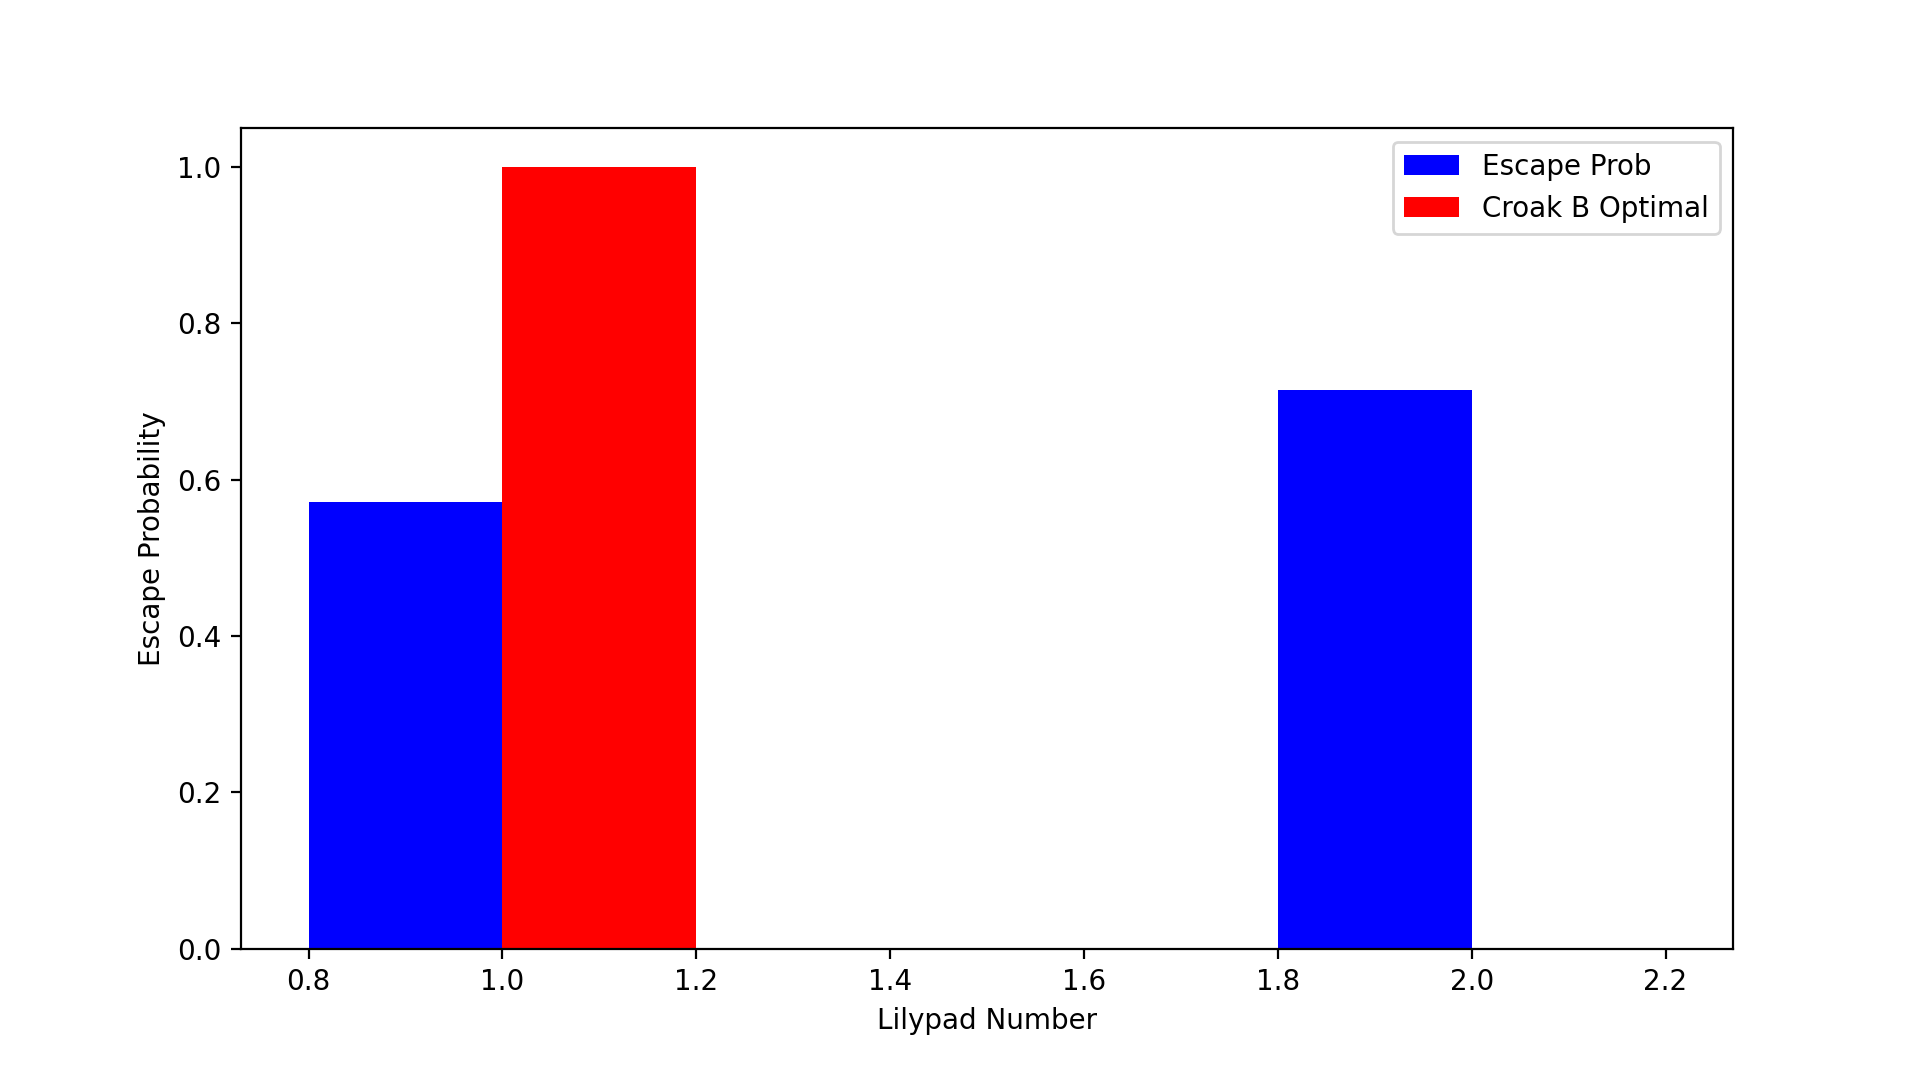
\includegraphics[width=\linewidth]{llp_3.png}
  \caption{Optimal Escape Probs and Optimal Policy}
  \label{fig:llp3}
\end{figure}

\begin{figure}
  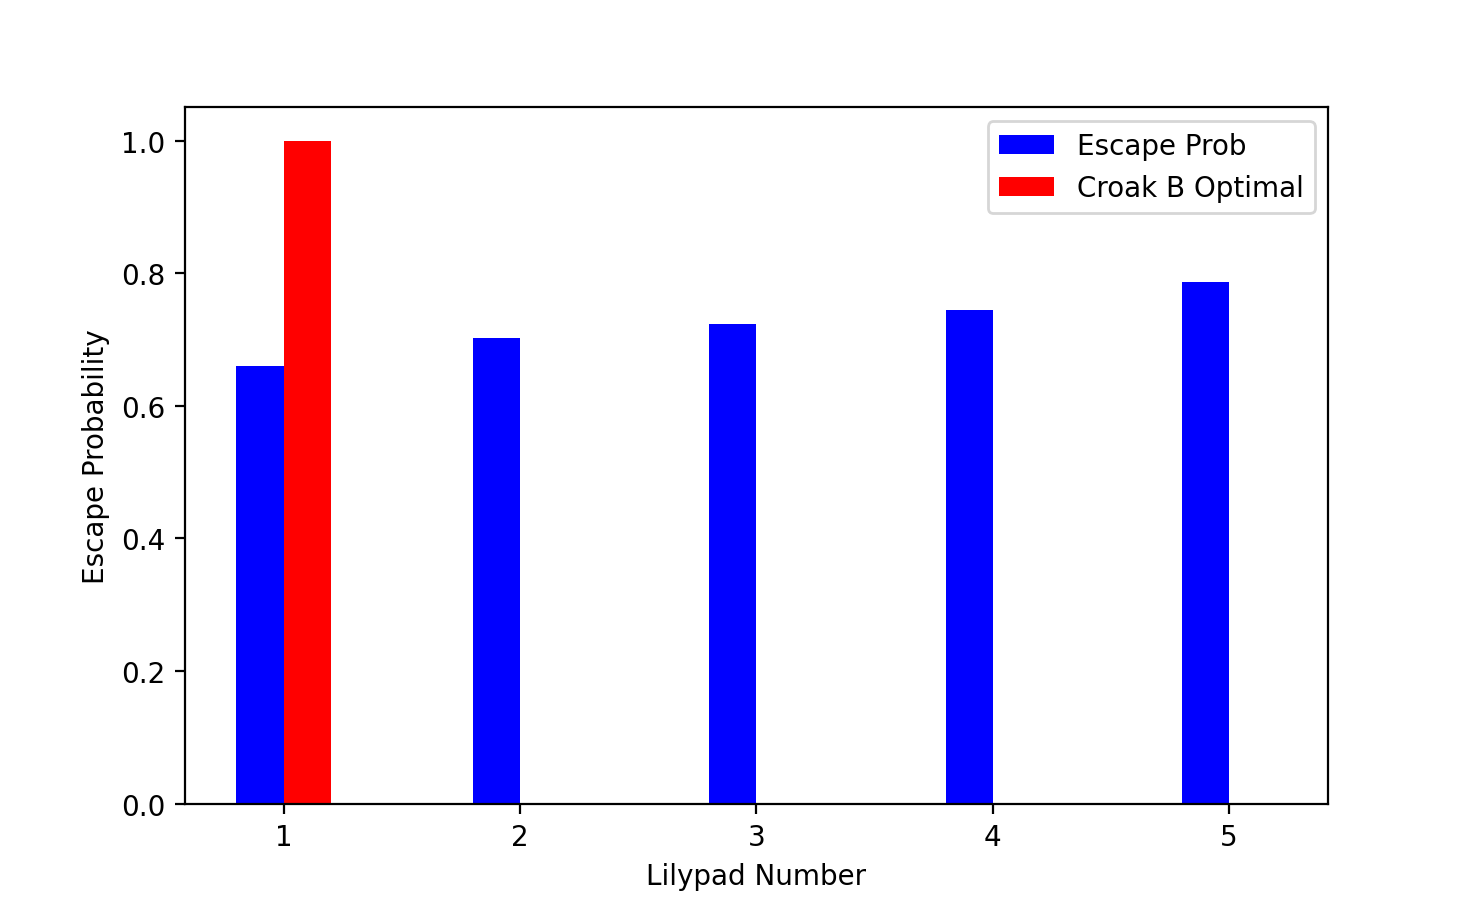
\includegraphics[width=\linewidth]{llp_6.png}
  \caption{Optimal Escape Probs and Optimal Policy}
  \label{fig:llp6}
\end{figure}

\begin{figure}
  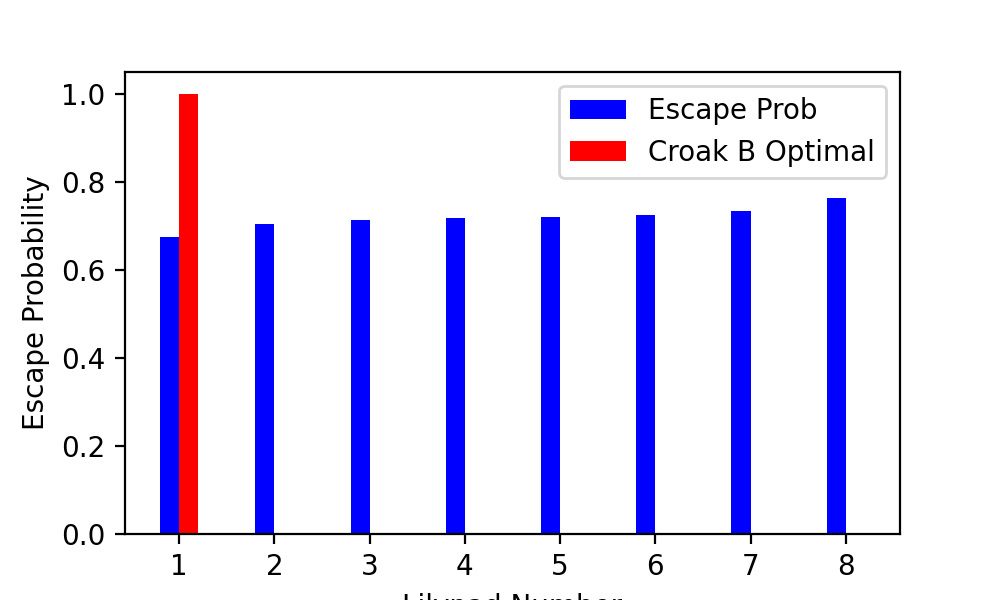
\includegraphics[width=\linewidth]{llp_8.png}
  \caption{Optimal Escape Probs and Optimal Policy}
  \label{fig:llp9}
\end{figure}

\section{Continuous Action Process}

We compute:
\begin{align*}
V(s) = E_s'[R(s') + 0V(s') | s,a] = E_s'-[e^{a,s'}]. = -M_x(a)
\end{align*}
In words, the cost function and transition probability means the value of a state is given by the negative of the moment generating function of a normal distribution of mean $s$ and variance $\sigma^2$ which is know to yield:
\begin{align*}
V(s) = e^{sa}e^{\frac{1}{2}\sigma^2 a^2}
\end{align*}
This quantity is minimized when its log is minimized so we must minimize $\frac{1}{2}\sigma^2a^2 + sa$ which is a quadratic expression known to obatin min at $a = \frac{-\sigma^2}{4s}$ yielding the the optimal value:
\begin{align*}
V^*(s) = e^{\frac{-\sigma^2}{4}}e^{\frac{1}{2}\sigma^2 \frac{-\sigma^4}{16s^2}} =  e^{\frac{-\sigma^2}{4}}e^{-\frac{1}{32} \frac{\sigma^6}{s^2}}
\end{align*}
\end{document}
